% !TEX encoding = UTF-8 Unicode
%!TEX root = thesis.tex
% !TEX spellcheck = en-US
%%=========================================
\chapter[Theoretical Background]{Theoretical Background} \label{ch:Theory}

Providing the needed background for all subsequent considerations, the current chapter outlines the concepts of numerical analysis and LCS theory used throughout this study. In particular, this pertains to solution of ordinary differential equations by use of Runge-Kutta methods, spline interpolation, finite strain theory, and the theoretical foundation of hyperbolic LCSs. Finally, the latter concepts will be used to pose existence criteria, as well as some key characteristics for hyperbolic LCSs.

%%==================================================================================
\section{Numerically solving ordinary differential equations}\label{sec:ODEs}

%When considering real world transport systems, accurate analysis is usually impeded either by lack of reliable data, lack of computational resources, or both. It is in the face of these challenges that utilizing Lagrangian coherent structures (LCSs) to gain some structural insight into the system becomes attractive. Moreover, the same complexity and limited understanding that motivates application of LCS theory also tends to prompt use of numerical interpolation and integration. 

Particle transport problems are often governed by sets of ordinary differential equations (ODEs) of the form

\begin{equation}\label{ODE}
	\dot{\vec{x}} = \vec{v}(t,\vec{x}),
\end{equation}

\noindent where $\vec{v}$ is the velocity field function, $t$ is time, and $\vec{x}$ and $\dot{\vec{x}}$ are the particle position and corresponding time derivative, respectively. Solving equation \eqref{ODE} amounts to finding $\vec{x}(t)$. As only a few exceptional ODE systems may be solved analytically, most cases require  numerical solution by use of a numerical ODE solver. The simplest and most intuitive of these is the Euler method

\begin{equation}\label{eq:Euler}
	\vec{x}_{n+1} = \vec{x}_n + \vec{v}(t_n,\vec{x}_n)\Delta t,
\end{equation}

\noindent where $t_n$ is the $n$\ts{th} time step and $\vec{x}_n$ is an approximation of $\vec{x}(t_n)$; the exact solution of equation \eqref{ODE} at time $t_n$. Note that $t_n = t_0 + n\Delta t$, where $t_0$ is the start time and $\Delta t$ is the time step length. Solving an ODE such as equation \eqref{ODE} numerically to find an approximation of $\vec{x}(t)$, is known as numerical integration of the ODE.

%%=========================================
\subsection{Runge-Kutta iterative ordinary differential equation solvers}\label{sec:RK}

Several of the most common numerical integrators are members of the Runge-Kutta family of explicit iterative methods. In the two-variable case (e.g. $t,x$), these methods are of the form

\begin{equation} \label{eq:RK}
	x_{n+1} = x_n + \Delta t(b_1k_1+...+b_s k_s).
\end{equation}

\noindent Here, $x_n$ and $x_{n+1}$ are the current and coming iterations of the function value, respectively. Intermediate time step slope evaluations are denoted by $k_i$, while $b_i$ are the corresponding weighting coefficients. The number of stages and order of the method are denoted $s$ and $p$, respectively. Note that in the case of ODEs, the two-variable case may easily be extended by treating multiple dependent variables separately.

The Runge-Kutta explicit iterative methods may be considered as a generalization of the classical 4\ts{th}-order Runge-Kutta method to any order. The 4\ts{th}-order classical Runge-Kutta method, for an ODE $\dot{x}=f(t,x)$, is given by

\begin{align} \label{eq:RK4a}
\begin{aligned}
	x_{n+1} &= x_n + \frac{\Delta t}{6}(k_1 +2k_2 + 2k_3 + k_4), \\
	t_{n+1} &= t_n + \Delta t, \\
	k_1 &= f(t_n,x_n), \\
	k_2 &= f(t_n + \frac{\Delta t}{2}, x_n + \frac{k_1}{2} \Delta t), \\
	k_3 &= f(t_n + \frac{\Delta t}{2}, x_n + \frac{k_2}{2} \Delta t), \\
	k_4 &= f(t_n + \Delta t,x_n + k_3 \Delta t),
\end{aligned}
\end{align} 

\noindent and is commonly used for a wide range of applications due to its 4\ts{th}-order accuracy, ease of implementation, and moderate computational requirements. Specifically, Runge-Kutta methods of order $p>4$ require a larger number of stages $s$ than their order, yielding a reduced accuracy gain per additional function evaluation \citep{SolvingODEs}. %Here, $f(t,x)$ is the time-derivative of the function $x(t)$, analogous to $\vec{v}(t,\vec{x})$ in equation \eqref{ODE}. %Note that a solution by the 4\ts{th}-order Runge-Kutta method requires access to $f(t_0 + \ n\Delta t/2,x)$ along the trajectory of $x$, where $n$ is any integer such that $t_0 +\ n\Delta t/2$ is within the considered time interval. 

%%=========================================
\subsection{Runge-Kutta method error bounds}\label{sec:RKerrorbounds}

Explicit Runge-Kutta methods of order $p$ are defined by their partial derivatives matching those of the underlying analytical solution up to and including order $p$ \citep{SolvingODEs}. This attribute has implications for their error bounds in a single step, usually referred to as local error. The local error $e(\Delta t)$ is defined as

\begin{equation} \label{eq:localerror}
	e(\Delta t) = x(t_0+\Delta t)-x_1,
\end{equation}

\noindent where $t_0$ may be identified as the time corresponding to the previous function value; $x(t_0)=x_0$. As outlined in \cite{Bieberbach51}, this may be analyzed by substituting equation \eqref{eq:RK} into equation \eqref{eq:localerror}

\begin{equation}
e(\Delta t) = x(t_0+\Delta t)-x_0-\Delta t\sum_{i=1}^{s}b_ik_i 
\end{equation}

\noindent and Taylor expanding

\begin{equation} \label{eq:Taylor_y}
x(t_0+\Delta t)=x_0+x'(t_0)\Delta t+x''(t_0)\frac{\Delta t^2}{2!}+\ldots+x^{(p+1)}(t_0+q\Delta t)\frac{\Delta t^{p+1}}{(p+1)!},
\end{equation}

\begin{equation} \label{eq:Taylor_k}
k_i(\Delta t) = k_i(0)+k_i'(0)\Delta t+\ldots+k_i^{(p)}(q_i\Delta t)\frac{\Delta t^p}{p!},
\end{equation}

\noindent with $0<q<1$ and $0<q_i<1$. Note that due to the partial derivatives up to and including order $p$ being identical, we are left with the terms in the Taylor expansions corresponding to $x$ and $k$ of orders including and exceeding $p+1$ and $p$, respectively.

Consequently, if a Runge-Kutta method of order $p$ is applied to a function $f(t,x)$ with existing and continuous partial derivatives up to order $p$, then the local error is strictly bounded by

\begin{equation} \label{localerrorbound1}
\left| x(t_0+\Delta t)-x_1 \right| \leq \Delta t^{p+1}\left( \frac{1}{(p+1)!}\max_{q\in [0,1]}\left|x^{(p+1)}(t_0+q\Delta t)\right| + \frac{1}{p!}\sum_{i=1}^{s}\left| b_i\right| \max_{q\in [0,1]}\left|k_i^{(p)}(q\Delta t)\right| \right),
\end{equation}

\noindent which gives

\begin{equation} \label{localerrorbound2}
\left|e(\Delta t)\right| = \left|x(t_0+\Delta t)-x_1\right| \leq C\Delta t^{p+1}
\end{equation}

\noindent for the order of the Runge-Kutta method local error, where $C$ is some constant.

Given the iterative nature of Runge-Kutta methods, the way in which their local error compounds into global error over $n$ consecutive time steps is of great interest. The global error of a numerical solution is the deviation from the analytical solution after several steps given by

\begin{equation}
	E = x(t_n)-x_n,
\end{equation}

\noindent where $x_n$ is obtained by $n$ successive iterative steps from $x_0$ and $x(t_n)$ is the analytical solution evaluated at $t_n$. As described in detail in \cite{SolvingODEs}; if the local error of an iteration of a Runge-Kutta method satisfies equation \eqref{localerrorbound2}, then we have for the global error

\begin{equation} \label{globalerror}
\left| E \right| \leq \tilde{C}\Delta t^p,
\end{equation}

\noindent where $\tilde{C}$ again is a constant, in general different from $C$.

\subsection{Adaptive step Runge-Kutta methods}\label{sec:adaptive_step}

The previously described ODE solvers are all constant step length methods. That is, we choose a step length, manually or otherwise, balancing accuracy requirements with performance restrictions. This step length is then used throughout the entire iterative solution, unless a step length change is explicitly specified. This is problematic as the local behavior of our target solution may require varying step lengths at different points in our computation. As we have no \textit{a priori} knowledge of this possibly changing local behavior, manually selecting an optimal step length is impractical.

The idea of adaptive step methods is to constantly estimate the local error of our chosen iterative solver. By defining a local error tolerance level $\epsilon_{\text{tol}}$, we can then evaluate whether the chosen step length was in fact adequate for this specific phase of our calculation. If the local error is estimated to exceed our tolerance level, we reject and recompute the current step with a shorter time step, while a comparatively small error prompts the solver to accept the step and increase the step length for the subsequent iteration.

An error estimate may be computed by using the same discretization method for two different step lengths. Alternatively, we may use one step length and two different Runge-Kutta discretization methods of orders $p$ and $p+1$. These are called \textit{Runge-Kutta-Fehlberg methods} \citep{NumericalAnalysis} and have the form

\begin{align}\label{eq:adaptive_step}
\begin{aligned}
\widehat{x}_{n+1} &= \bar{x}_n + \Delta t\phi_{\Romannum{1}}(t_n,\bar{x}_n;\Delta t),\\
\bar{x}_{n+1} &= \bar{x}_n + \Delta t\phi_{\Romannum{2}}(t_n,\bar{x}_n;\Delta t),
\end{aligned}
\end{align}

\noindent where $\phi_{I}(t_n,\bar{x}_n;\Delta t)$ and $\phi_{II}(t_n,\bar{x}_n;\Delta t)$ are Runge-Kutta methods of order $p$ and $p+1$, respectively. We implement step length control by considering the difference

\begin{equation}\label{eq:step_control_diff_1}
\bar{x}_{n+1} - \widehat{x}_{n+1} = \Delta t\big( \phi_{\Romannum{2}}(t_n,\bar{x}_n;\Delta t)- \phi_{\Romannum{1}}(t_n,\bar{x}_n;\Delta t)\big).
\end{equation}

\noindent It follows from equation \eqref{localerrorbound2} that $\phi_{\Romannum{1}}$ and $\phi_{\Romannum{2}}$ have local errors of order $p$ and $p+1$, respectively. We may therefore, for small $\Delta t$, express the difference in equation \eqref{eq:step_control_diff_1} as

\begin{equation}\label{eq:step_control_diff_2}
\bar{x}_{n+1} - \widehat{x}_{n+1} \approx C(t_n)\Delta t^{p+1},
\end{equation}

\noindent where $C(t)$ is some function. Neglecting higher order error terms, we now use equation \eqref{eq:step_control_diff_2} as an approximation for the local error associated with using $\phi_{\Romannum{1}}(t_n,\bar{x}_n;\Delta t)$.

Suppose that we just completed a successful step, that is, we have

\begin{equation}\label{eq:step_condition}
\left|\bar{x}_{n+1}-\widehat{x}_{n+1}\right| \approx \left|C(t_n)\Delta t^{p+1}\right| \leq \epsilon_{\text{tol}}.
\end{equation}

\noindent Now, by assuming 

\begin{equation}
C(t_n)\approx C(t_{n+1}) \approx \frac{\left| \bar{x}_{n+1} - \widehat{x}_{n+1}\right|}{\left| \Delta t^{p+1}\right|},
\end{equation}

\noindent we can approximate our condition \eqref{eq:step_condition} by

\begin{equation}
\left| \bar{x}_{n+1} - \widehat{x}_{n+1}\right|\left|\frac{\Delta t_{\text{new}}}{\Delta t}\right|^{p+1} \leq \epsilon_{\text{tol}}.
\end{equation}

\noindent Finally, we estimate the new step length by isolating $\Delta t_{\text{new}}$ according to

\begin{equation}\label{eq:dt_new}
\Delta t_{\text{new}} = \Delta t\left|\frac{\epsilon_{\text{tol}}}{\bar{x}_{n+1} - \widehat{x}_{n+1}}\right|^{1/(p+1)}.
\end{equation}

Whether $\bar{x}$ or $\widehat{x}$ is used for the actual solution step depends on the particular method implementation. Several adaptive step methods are available in literature. The widely used Dormand-Prince method of orders $p=4$ and $5$ is outlined by for example \cite{NumericalAnalysis} and \cite{Dormand-Prince1980}. A higher order alternative, corresponding to orders $p=7$ and $8$, is described by \cite{Dormand-Prince1981}.

%%=========================================
\subsection{Interpolation}\label{sec:SplineInterpolation}

Given that real world transport systems are known only by partial measurement or grid based model output, considering the trajectories of particles moving between these sampling or grid points necessitates use of interpolation. A two-dimensional interpolation problem may be described by considering the family of functions

\begin{equation}\label{eq:Phi}
	\Phi (x,y;a_0,\ldots,a_n),
\end{equation}

\noindent each characterized by the $n+1$ parameters $a_0,\ldots ,a_n$. Having been given a set of $n+1$ coordinates and corresponding function values $(x_i,y_i,f_i)$, where $x_i\neq x_k$ for $i\neq k$ and $f_i=f(x_i,y_i)$, the interpolation problem amounts to determining the set of parameters $\{a_i\}_{i=0}^n$ as to make $\Phi$ satisfy

\begin{equation}\label{eq:ItpProblem}
	\Phi(x_i,y_i;a_0,\ldots,a_n) = f_i, \quad i = 0,...,n.
\end{equation}

\noindent Here, we name the coordinates $(x_i,y_i)$, function values $(f_i)$, and points $(x_i,y_i,f_i)$ support abscissas, support ordinates, and support points, respectively. Moreover, as long as $\Phi$ depends linearly on the set of parameters $a_i$, and may be written in the form

\begin{equation}\label{eq:LinearItpProblem}
	\Phi (x,y;a_0,...,a_n) = a_0\Phi_0(x,y) + a_1\Phi_1(x,y) +...+ a_n\Phi_n(x,y),
\end{equation}

\noindent this may be classified as a linear interpolation problem. According to \cite{NumericalAnalysis}, the linear class of interpolation problems includes among others polynomial interpolation, trigonometric interpolation, and spline interpolation.

An interpolation problem is solved through spline interpolation by determining the set of parameters $\{a_i\}_{i=0}^n$ in equation \eqref{eq:LinearItpProblem} with the set of corresponding functions $\{\Phi_i\}_{i=0}^n$ limited to spline functions. These spline functions, also simply referred to as splines, are connected by use of a partition. Considering the one-dimensional case for simplicity, the partition

\begin{equation}
	\Delta:\quad a=x_0<x_1<...<x_n=b
\end{equation}

\noindent of the interval $[a,b]$ gives the domains of the piecewise polynomial spline functions $S$ in the set $S_{\Delta}$. These spline functions are connected at support abscissas, in the context of splines called knots. Order $k$ spline functions $S_k$ may be defined as piecewise polynomial functions of order $k$ that are $k-1$ times differentiable at all interior knots of $\Delta$ (that is, $x_i$ for $1\leq i\leq n-1$) \citep{NumericalAnalysis}. These spline functions are entirely defined by their $k+1$ coefficients, determined by the $k-1$ derivatives and the function value at their left bordering knot, as well as the function value at their right bordering knot. In order to properly define splines in the exterior subdomains $[x_0,x_1]$ and $[x_{n-1},x_n]$, we impose boundary conditions. As the splines are composed of polynomials, the $k-1$ times differentiability condition at each knot ensures the resulting spline interpolation $\Phi$ is $k-1$ times differentiable at all points. 

A special class of these piecewise polynomial functions, B-splines have some very useful properties. That is, B-splines are nonnegative and evaluate to zero everywhere except the contiguous interval $[x_i,x_{i+1}]$ \citep{NumericalAnalysis}. This makes B-splines ideal for spline interpolation.

A selection of spline interpolators applied to a discretely sampled 5\ts{th}-order polynomial is displayed in figure \ref{fig:Splines}, highlighting the increased accuracy of higher order splines when applied to continuous functions. Higher order spline interpolation schemes do however require more input. Specifically, a $k$\ts{th} order spline requires at least $k+1$ input coordinates. According to \cite{NumericalAnalysis}, spline functions have seen increasing use in numerical methods due to yielding smooth interpolating curves with a limited prevalence of oscillations for higher order polynomials.

%As may be inferred from figure \ref{fig:Splines}, the spline interpolation of order $5$ is exact for this 5\ts{th}-order polynomial. In fact, any spline interpolation of order $k$ is exact for all polynomials of order $l\leq k$.

\begin{figure}[h!] 
\centering
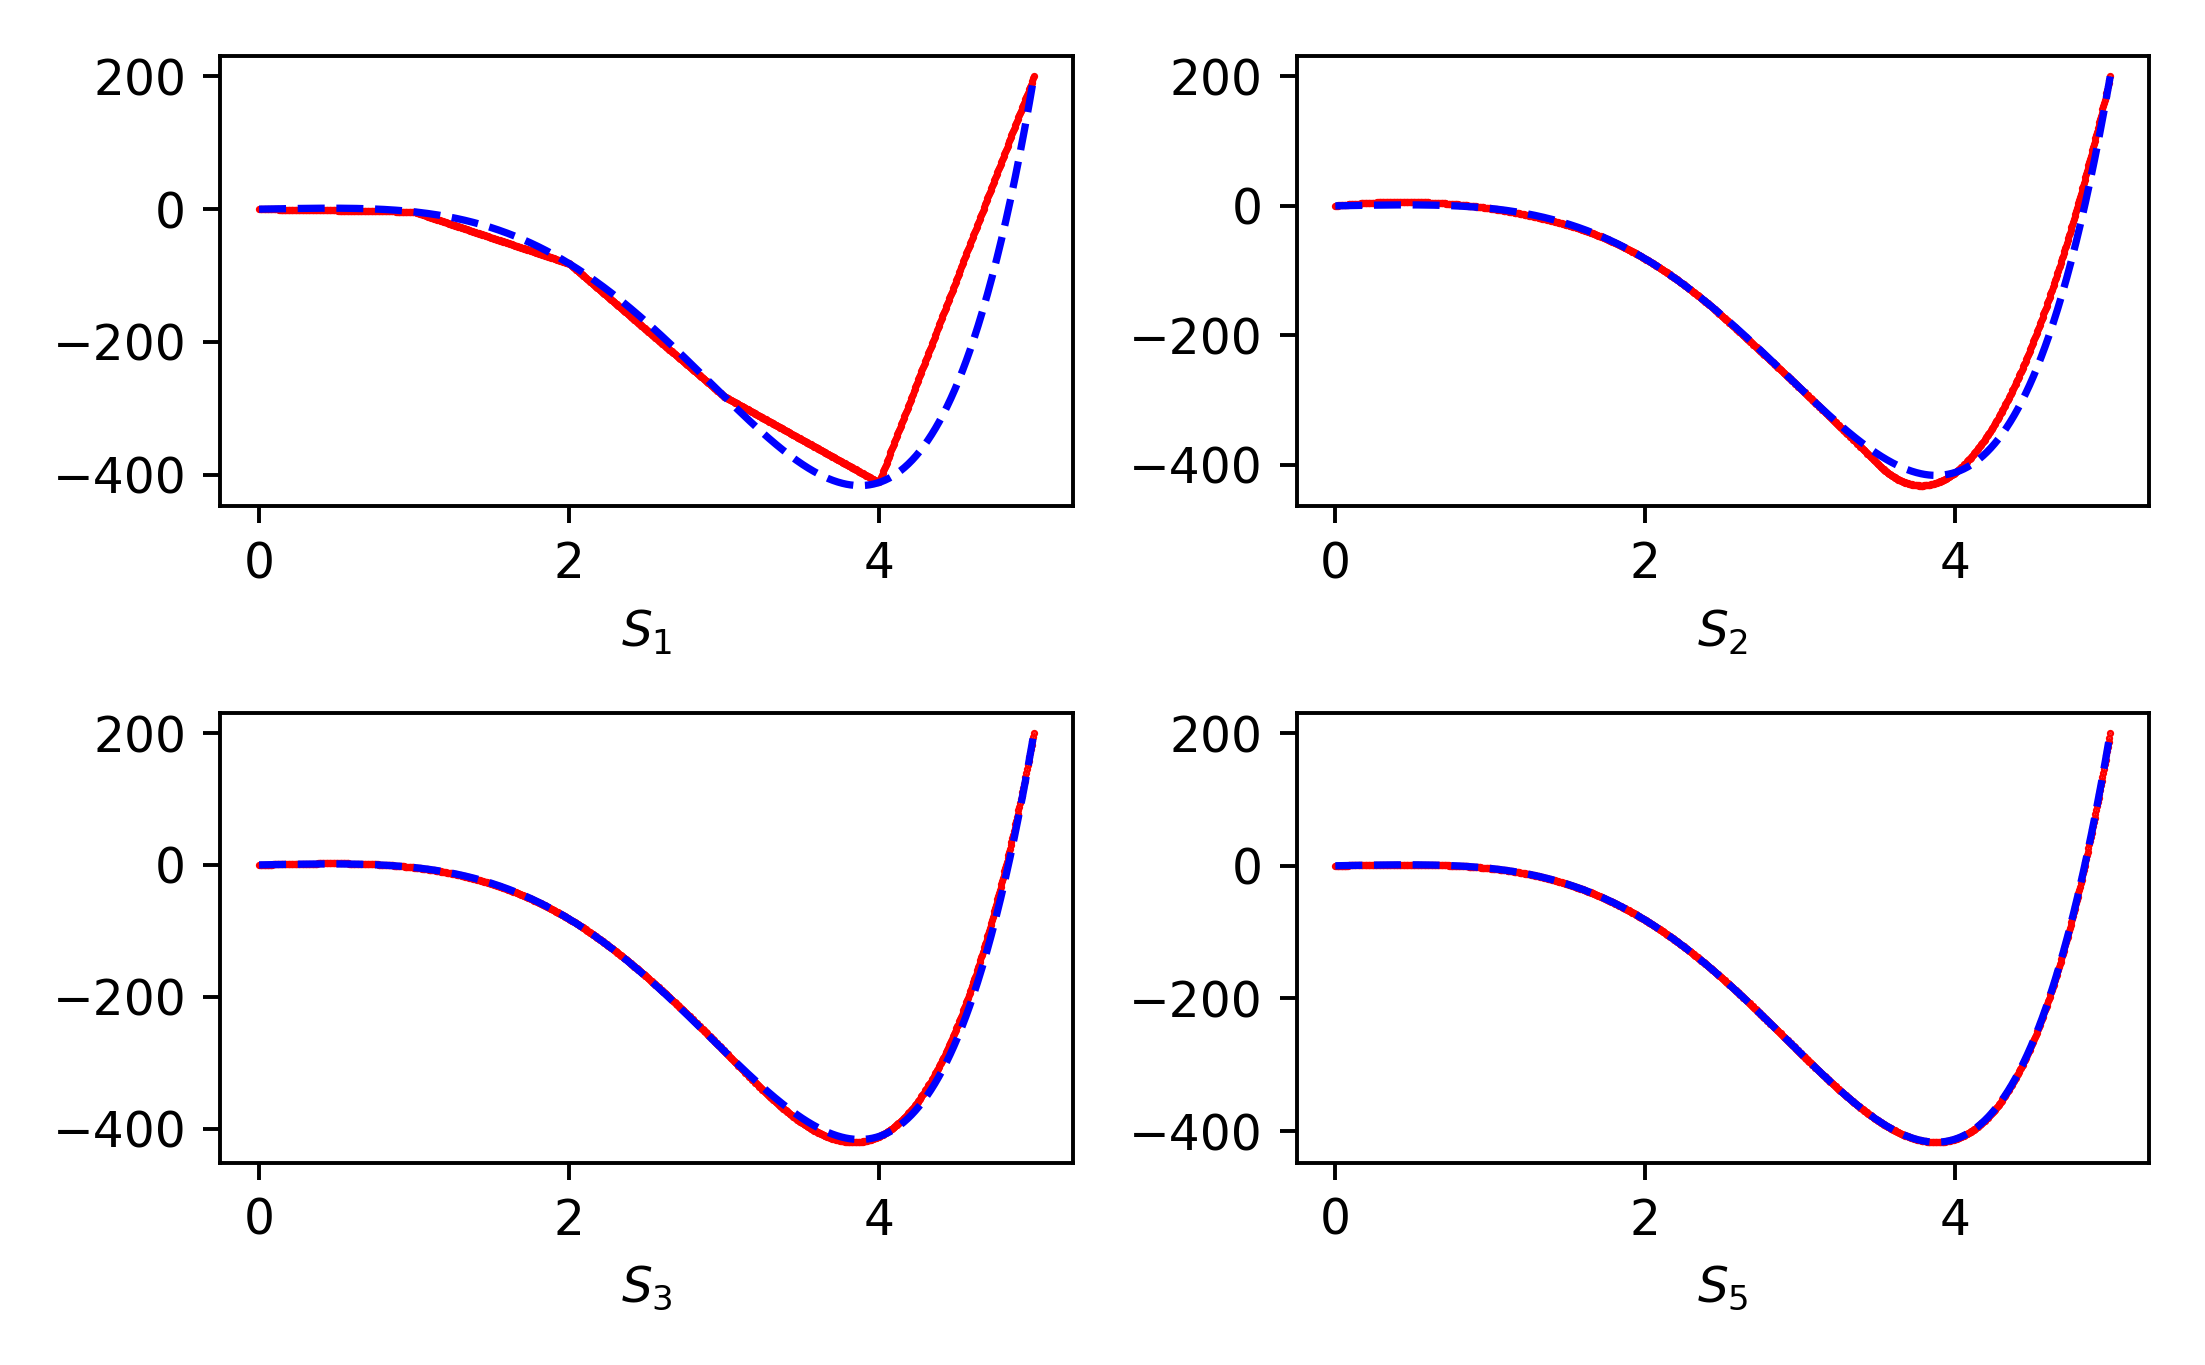
\includegraphics{fig/Splines.png}
\caption{Spline interpolation of orders 1, 2, 3, and 5 in solid red applied to a discretely sampled fifth order polynomial (blue dashed line). We observe that higher order splines yield more accurate interpolations.}
\label{fig:Splines}
\end{figure}

%%===============================================
%\subsection{Applying Runge-Kutta iterative solvers to splines}\label{sec:RKITPinteraction}

%To our knowledge, no available theory exists for the error bounds of order $p$ Runge-Kutta methods applied to ODE systems without continuous derivatives up to order $p$ yielding error bounds of rigor equivalent to equation \eqref{localerrorbound1}. Considering the strict error bounds obtainable from equation \eqref{localerrorbound1}, it therefore seems prudent to use the differentiability of the underlying system as a guide to selection of iterative method. In other words, given that balancing computational demands against limiting numerical error is the primary concern of method selection, it seems reasonable to choose a Runge-Kutta method of order matching the differentiability of the ODE system. Specifically, if the first $p$ derivatives of the ODE system are continuous, choosing a Runge-Kutta method of order higher than $p$ does not necessarily yield a more accurate solution. Conversely, choosing a Runge-Kutta method of order lower than $p$ likely amounts to forfeiting system accuracy.

%In the context of applying Runge-Kutta methods to spline-interpolated ODE systems, we may therefore expect that matching the orders of the Runge-Kutta method with that of the spline interpolation will yield a favorable balance between computational requirements and numerical accuracy.

%%==================================================================================
\section{Transport systems}\label{sec:TransportSystems}

LCS theory may be seen as a set of tools developed to gain useful insight into finite-time transport systems that may be too sensitive to initial conditions to be accurately described by conventional numerical modelling. Correspondingly, LCS theory deals with the transport of passive tracers in velocity fields. Tracers are infinitesimal particles that follow the currents of the system without influencing it, or each other, in any way. The underlying velocity field is usually given, as the method by which this is obtained is inconsequential to the characteristics of the system. Although the scope of the current investigation primarily treats the three-dimensional case, considering the more well-known two-dimensional case is useful in terms of outlining theoretical concepts.

\subsection{Transport system description and notation}

Consider a transport problem in a finite-time three-dimensional unsteady velocity field of the form

\begin{equation}\label{eq:System}
	\dot{\vec{x}} = \vec{v}(t,\vec{x}), \quad \vec{x}\in U,\quad t\in [ t_0, t_0+T],
\end{equation}

\noindent where $\vec{x}$ is position, $t$ denotes time, $\vec{v}$ is the velocity field function, $U$ is the function domain, and $t_0$ and $t_0+T$ are the start and stop times, respectively. Considering a particle in the system \eqref{eq:System} of initial position $\vec{x}(t_0)=\vec{x}_0$, we denote its subsequent trajectory by

\begin{equation}\label{eq:Trajectory}
	\vec{x}(t;t_0,\vec{x}_0).
\end{equation}

\noindent We then define the flow map $\vec{F}_{t_0}^t$ as

\begin{equation}\label{eq:Flowmap}
	\vec{F}_{t_0}^t(\vec{x}_0) \coloneqq \vec{x}(t;t_0,\vec{x}_0),
\end{equation}

\noindent mapping the set of initial positions in $U$ at time $t_0$ to the corresponding positions at time $t$. As noted in \cite{LCSreview}, the flow map retains the smoothness of the underlying velocity field.

\subsection{Deformation}\label{sec:Deformation}

As a set of passive tracer particles are transported, neighboring particles are likely to either diverge or converge at various rates based on the local properties of the velocity field. These local rates of repulsion or attraction may be described and quantified by considering the flow maps of particles with nearly identical initial conditions. Specifically, we consider the flow map three-dimensional Jacobian, or flow gradient, given by

\begin{equation}\label{eq:Jacobian}
	\nabla \vec{F}_{t_0}^t(\vec{x}_0) =
	\begin{bmatrix}
		\dfrac{\partial x}{\partial x_0} & \dfrac{\partial x}{\partial y_0} & \dfrac{\partial x}{\partial z_0} \\[2ex]
		\dfrac{\partial y}{\partial x_0} & \dfrac{\partial y}{\partial y_0} & \dfrac{\partial y}{\partial z_0} \\[2ex]
		\dfrac{\partial z}{\partial x_0} & \dfrac{\partial z}{\partial y_0} & \dfrac{\partial z}{\partial z_0}
	\end{bmatrix},
\end{equation}

\noindent where $\frac{\partial}{\partial x_0}$ etc. denotes differentiation with respect to initial position. The flow map Jacobian provides a measure for the local strain of the set of tracer initial positions.

Consider a small perturbation or initial position deviation $\bm{\epsilon}(t) = \vec{x}_2(t)-\vec{x}_1(t)$. Taking the time derivative given by equation \eqref{eq:System} with positions expressed by equation \eqref{eq:Trajectory} and using the Jacobian of the velocity field, we get

\begin{equation}\label{eq:EpsilonDot}
	\dot{\bm{\epsilon}} = \nabla \vec{v}(t,\vec{x}(t;t_0,\vec{x}_0)) \bm{\epsilon}.
\end{equation}

\noindent According to \cite{LCSreview}, this perturbation may be expressed as

\begin{equation}\label{eq:epsilon_of_t}
	\bm{\epsilon}(t) = \nabla \vec{F}_{t_0}^t(\vec{x}_0) \bm{\epsilon}(t_0),
\end{equation}

\noindent seeing as $\nabla \vec{F}_{t_0}^t(\vec{x}_0)$ is the fundamental matrix solution of equation \eqref{eq:EpsilonDot}. We therefore obtain, for the squared magnitude of the perturbation, at time $t$

\begin{equation}
	|\bm{\epsilon}(t)|^2 = \langle \nabla\vec{F}_{t_0}^t(\vec{x}_0) \bm{\epsilon}(t_0),\nabla\vec{F}_{t_0}^t(\vec{x}_0) \bm{\epsilon}(t_0)\rangle,
\end{equation}

\noindent where $\langle \vec{A},\vec{B}\rangle$ signifies taking the inner product of $\vec{A}$ and $\vec{B}$. This allows us to define the right Cauchy-Green strain tensor $\vec{C}_{t_0}^t(\vec{x}_0)$ as \citep{Truesdell&Noll}

\begin{equation} \label{eq:Cauchy-Green}
	\vec{C}_{t_0}^{t}(\vec{x}_0) = \left[ \nabla \vec{F}_{t_0}^{t}(\vec{x}_0)		\right]^* \vec{\nabla}\vec{F}_{t_0}^{t}(\vec{x}_0),
\end{equation}

\noindent yielding

\begin{equation}
	|\bm{\epsilon}(t)|^2 = \left\langle \bm{\epsilon}(t_0), \vec{C}_{t_0}^{t}(\vec{x}_0)\bm{\epsilon}(t_0) \right\rangle,
\end{equation}

\noindent where $[...]^*$ signifies matrix transposition. Hence, the Cauchy-Green strain tensor maps position perturbations at time $t_0$ to their magnitudes at a later time $t$. Due to the invertibility of $\nabla \vec{F}_{t_0}^t(\vec{x}_0)$, the Cauchy-Green strain tensor is positive definite \citep{LCSreview}. Furthermore, in three dimensions, it satisfies the following eigenvector and eigenvalue relations:


\begin{align}\label{eq:CGRelations}
\begin{aligned}
	\vec{C}_{t_0}^{t}(\vec{x}_0)\bm{\xi}_i(\vec{x}_0) = \lambda_i(\vec{x}_0)				\bm{\xi}_i(\vec{x}_0&), \quad |\bm{\xi}_i(\vec{x}_0)| = 1, \quad i=1,2,3,  \\
	0 < \lambda_1(\vec{x}_0) \leq& \lambda_2(\vec{x}_0) \leq \lambda_3(\vec{x}_0), \\
	\bm{\xi}_1(\vec{x}_0)& \perp \bm{\xi}_2(\vec{x}_0),\\
	\bm{\xi}_1(\vec{x}_0)& \perp \bm{\xi}_3(\vec{x}_0),\\
	\bm{\xi}_2(\vec{x}_0)& \perp \bm{\xi}_3(\vec{x}_0),
\end{aligned}
\end{align}

\noindent where $\lambda_i$ and $\bm{\xi}_i$ are the eigenvalues and eigenvectors of $\vec{C}_{t_0}^{t}$, respectively \citep{Haller14}. The dependence of $\lambda_i$ and $\bm{\xi}_i$ on $t$ and $t_0$ has been omitted in the interest of notational simplicity. Note that these quantities describing material deformation satisfy objectivity (see section \ref{sec:LCS}). Moreover, for incompressible flow systems ($\text{div}(\vec{v})\equiv 0$), the eigenvalues of $\vec{C}_{t_0}^{t}(\vec{x}_0)$ also satisfy

\begin{equation}
	\lambda_1(\vec{x}_0)\lambda_2(\vec{x}_0)\lambda_3(\vec{x}_0) = 1
\end{equation}

\noindent for all $\vec{x}_0$ \citep{LCSreview}.

\subsection{Flow map dynamics}\label{sec:FlowMapDynamics}

The flow map $\vec{F}_{t_0}^{t}(\vec{x}_0)$ obeys

\begin{equation}\label{eq:var_eq_1}
\frac{\text{d}}{\text{d}t}\vec{F}_{t_0}^{t}(\vec{x}_0) = \vec{v}\left(t,\vec{F}_{t_0}^{t}(\vec{x}_0)\right),
\end{equation}

\noindent as tracer positions move in the velocity field $\vec{v}$. Useful for analyzing local deformation, the time development of the Jacobian of the flow map $\nabla \vec{F}_{t_0}^{t}(\vec{x_0})$ (see equation \eqref{eq:Jacobian}) is governed by \citep{VariationalEquations}

\begin{equation}\label{eq:var_eq_2}
\frac{\text{d}}{\text{d}t}\nabla \vec{F}_{t_0}^{t}(\vec{x_0}) = \nabla \vec{v}\left(t,\vec{F}_{t_0}^{t}(\vec{x_0})\right)\nabla \vec{F}_{t_0}^{t}(\vec{x_0}).
\end{equation}

\noindent In Cartesian coordinates, equation \eqref{eq:var_eq_2} constitutes 9 equations, each coupled with the three equations corresponding to equation \eqref{eq:var_eq_1}. Note that equation \eqref{eq:var_eq_2} may be expressed in Cartesian form as

\begin{equation}\label{eq:var_eq_2_cartesian}
\frac{\text{d}}{\text{d}t}\left(\frac{\partial F_i}{\partial x_j}\right) = \sum_k \frac{\partial v_i}{\partial x_k} \frac{\partial F_k}{\partial x_j}.
\end{equation}

\noindent Combined, equations \eqref{eq:var_eq_1} and \eqref{eq:var_eq_2_cartesian} form a system of $12$ coupled equations, solvable by ordinary ODE methods. 

%==============================
\subsection{Singular-value decomposition}\label{sec:SVD}

Computing the Cauchy-Green strain tensor $\vec{C}_{t_0}^t(\vec{x}_0)$ eigenvectors and eigenvalues constitutes a problem of the form

\begin{equation}\label{eq:eigen_problem}
\vec{B}^*\vec{B}\vec{Q} = \vec{Q}\vec{\Lambda},
\end{equation}

\noindent where $\vec{\Lambda}$ is the diagonal matrix 

\begin{equation}
	\vec{\Lambda} =
	\begin{bmatrix}
		\lambda_1 & 0 & 0 \\[2ex]
		0 & \lambda_2 & 0 \\[2ex]
		0 & 0 & \lambda_3
	\end{bmatrix}.
\end{equation}

\noindent Here, $\lambda_i$ are the eigenvalues of $\vec{B}^*\vec{B}$, where $\vec{B}$ is some $3\times 3$ matrix. Moreover, $\vec{Q}$ is another $3\times 3$ matrix, its $i$\ts{th} column corresponding to the $i$\ts{th} eigenvector of $\vec{B}^*\vec{B}$, denoted $\bm{\xi}_i$. This problem may be solved directly by computing $\vec{B}^*\vec{B}$ and finding its eigenvalues and eigenvectors. However, according to \cite{Watkins05}, some information about the smaller eigenvalues is lost when computing $\vec{B}^*\vec{B}$ in floating-point arithmetic. Instead, \cite{Watkins05} suggests utilizing singular-value decomposition.

Singular-value decomposition may be seen as a generalization of eigendecomposition. That is, as the eigendecomposition

\begin{equation}\label{eq:eigendecomposition}
\vec{B}^*\vec{B} = \vec{Q}\vec{\Lambda}\vec{Q}^{-1},
\end{equation}

\noindent follows from \eqref{eq:eigen_problem}, the more general singular-value decomposition follows from the relation

\begin{equation}
\vec{B}\vec{v}_i = \sigma_i\vec{u}_i.
\end{equation}

\noindent Here, $\sigma_i$ is the $i$\ts{th} singular value of $\vec{B}$, while $\vec{v}_i$ and $\vec{u}_i$ are the corresponding normalized right and left singular vectors. This relation may also be rewritten as 

\begin{equation}\label{eq:singular_problem}
\vec{B}\vec{V} = \vec{U}\vec{\Sigma}, 
\end{equation}

\noindent where $\vec{v}_i$ and $\vec{u}_i$ form the $i$\ts{th} columns of the orthogonal matrices $\vec{V}$ and $\vec{U}$, respectively. Note that for any orthogonal matrix $\vec{A}$, we have $\vec{A}^*=\vec{A}^{-1}$. Moreover, $\vec{\Sigma}$ is of the form

\begin{equation}
	\vec{\Sigma} =
	\begin{bmatrix}
		\sigma_1 & 0 & 0 \\[2ex]
		0 & \sigma_2 & 0 \\[2ex]
		0 & 0 & \sigma_3
	\end{bmatrix},
\end{equation}

\noindent where $\sigma_i$ are the positive and real singular values of $\vec{B}$ \citep{trefethen97}. As $\vec{V}$ is orthogonal, we may multiply equation \eqref{eq:singular_problem} by its inverse $\vec{V}^*$ from the right to obtain

\begin{equation}\label{eq:singular_value_decomposition}
\vec{B} = \vec{U}\vec{\Sigma}\vec{V}^*.
\end{equation}

This factorization corresponds to the most commonly used form of singular-value decomposition (SVD) \citep{trefethen97}. Now, consider our problem of computing the eigenvalues and eigenvectors of $\vec{B}^*\vec{B}$. By insertion of equation \eqref{eq:singular_value_decomposition}, we get

\begin{equation}\label{eq:B*B}
\vec{B}^*\vec{B} = \vec{V}\vec{\Sigma}^*\vec{U}^*\vec{U}\vec{\Sigma}\vec{V}^* =
\vec{V}(\vec{\Sigma}^*\vec{\Sigma})\vec{V}^*, 
\end{equation}

\noindent where we used that $\vec{U}^*\vec{U}=\vec{I}$ for the orthogonal matrix $\vec{U}$. Consequently, we may identify the eigenvalues $\lambda_i$ of $\vec{B}^*\vec{B}$ as $\sigma_i^2$. Moreover, by comparison of equation \eqref{eq:B*B} with equations \eqref{eq:eigendecomposition} and \eqref{eq:eigen_problem}, we notice that the columns of $\vec{V}$ correspond to the eigenvectors of $\vec{B}^*\vec{B}$.

Therefore, by performing singular-value decomposition on the matrix $\vec{B}$, we are able to implicitly compute the eigenvalues and eigenvectors of $\vec{B}^*\vec{B}$. As this is done without actually computing $\vec{B}^*\vec{B}$, we limit numerical error due to use of floating-point arithmetic. In the context of deformation, this means that we may use $\vec{\nabla}\vec{F}_{t_0}^{t}(\vec{x}_0)$ to compute the eigenvalues and eigenvectors of $\vec{C}_{t_0}^{t}(\vec{x}_0) = \left[ \nabla \vec{F}_{t_0}^{t}(\vec{x}_0)\right]^* \vec{\nabla}\vec{F}_{t_0}^{t}(\vec{x}_0)$ directly.
%%==================================================================================
\section{Hyperbolic Lagrangian coherent structures} \label{sec:LCS}

Inspired by coherent tracer patterns observed both experimentally and in nature, Lagrangian coherent structure (LCS) theory emerged in the interface between nonlinear dynamics and fluid mechanics as an alternative way of approaching and understanding transport in complex fluid flow systems. Coined by \cite{HallerandYuan}, the term Lagrangian coherent structure refers to the most repelling, attracting or shearing material surfaces that guide the principal structures of particle transport dynamics \citep{LCSreview}. Here, material surfaces refer to time-evolving structures in a flow system, traceable by a set of particles following the set of point trajectories defining the surface. As necessitated by their material surface nature, LCS theory takes a Lagrangian perspective where the identities of individual particles are tracked as they are advected in a velocity field. This is opposed to the Eulerian perspective, where we consider the behavior of the flow field at stationary points in space. Here, particles are simply viewed as realizations of the velocity field as they pass points in space, their identities therefore irrelevant.

The concept of objectivity is also central to the development of LCS theory. Objectivity is one of the fundamental axioms of mechanics and requires that any material response is independent of the perspective of the observer. This makes it necessary to for example take centrifugal forces and the Coriolis effect into account when calculating flow velocity fields on a rotating planet. 

Motivated by application in real world systems, LCS theory deals exclusively with finite-time systems. Here, asymptotic concepts from nonlinear dynamics such as stable and unstable manifolds lose their meaning, necessitating the use of finite-time tools. The three main types of LCSs; hyperbolic, elliptic and parabolic, are examples of such finite-time tools used to gain insights into overarching flow patterns. According to \cite{LCStool}, hyperbolic LCSs are defined as the locally most repelling or attracting material surfaces in a specific time interval $[t_0,t]$. One useful property of these attracting and repelling LCSs is forward-backward time duality. As described by \cite{LCSreview}, this permits us to compute attracting and repelling LCSs using the same time interval $[t_0,t]$. In the case of repelling LCSs, this is done by ordinary advection, while attracting LCSs are computed by use of a reversed flow map attained from backward-time advection.

Unlike hyperbolic LCSs, elliptic LCSs and parabolic LCSs are described as coherent Lagrangian vortex boundaries and Lagrangian jet cores, respectively \citep{LCStool}. However, all LCSs may be seen as consisting of a set of particles evolving with the particle transport in time, like any other material surface.

%%=========================================
\subsection{Defining most repelling material surfaces}\label{sec:MostRepelling}

Focusing on hyperbolic LCSs, we now follow the argument of \cite{Haller12} endeavoring to quantify normal attraction and repulsion for a smooth curve $\mathcal{M}(t_0)$ at time $t_0$ in a two-dimensional system. This is motivated by the previously discussed definition of hyperbolic LCSs as locally most repelling or attracting material surfaces. While the main focus of our discussion pertains to three-dimensional systems, the two-dimensional case is useful in terms of coherently outlining this underlying argument. 

As the system evolves, the material line $\mathcal{M}(t_0)$ is transported according to the flow map forming a time-dependent material line $\mathcal{M}(t) = \vec{F}_{t_0}^t(\mathcal{M}(t_0))$. Now, choose a normal vector $\vec{n}_0$ for each initial position $\vec{x}_0 \in \mathcal{M}(t_0)$, as visualized in figure \ref{fig:UnitNormal}\textcolor{blue}{a}.

\begin{figure}[h!] 
\centering
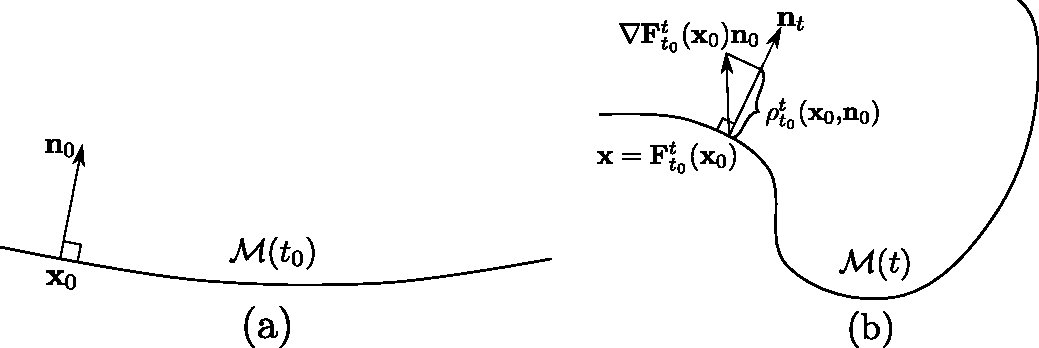
\includegraphics[width=14cm]{fig/UnitNormal.pdf}
\caption{Visualization of the repulsion rate $\rho_{t_0}^t(\vec{x}_0,\vec{n}_0)$ for $\vec{x}_0$ on the material line $\mathcal{M}(t_0)$. (a) $\vec{n}_0$ denotes the normal vector of the material line $\mathcal{M}(t_0)$ at the point $\vec{x}_0$. (b) The vector $\vec{\nabla}\vec{F}_{t_0}^t(\vec{x}_0)\vec{n}_0$ indicates how $\vec{n}_0$ has evolved in the time interval $[t_0,t]$, as defined by the advection of the particles initially situated at its endpoints. The normal repulsion rate $\rho_{t_0}^t(\vec{x}_0,\vec{n}_0)$ is then defined by the component of this time-evolved vector that is normal to the advected material line $\mathcal{M}(t)$. The normal of $\mathcal{M}(t)$ is denoted $\vec{n}_t$.}
\label{fig:UnitNormal}
\end{figure} 

By considering the separation of the particles with initial positions $\vec{x}_0$ and $\vec{x}_0 + \vec{n}_0$, the time evolution of $\vec{n}_0$ is given by $\nabla \vec{F}_{t_0}^t(\vec{x}_0)(\vec{x}_0+\vec{n}_0 - \vec{x}_0) = \vec{\nabla}\vec{F}_{t_0}^t(\vec{x}_0)\vec{n}_0$ (see equation \eqref{eq:epsilon_of_t}). In order to measure the normal repulsion rate of the material line $\mathcal{M}(t_0)$, we are then interested in the component of this time-evolved normal vector that is perpendicular to $\mathcal{M}(t)$. Denoting this component $\rho_{t_0}^t(\vec{x}_0,\vec{n}_0)$, we may express the normal repulsion rate of $\mathcal{M}(t)$ on the trajectory $\vec{x}(t;t_0,\vec{x}_0)$ as

\begin{equation}
	\rho_{t_0}^t(\vec{x}_0,\vec{n}_0) = \frac{\left\langle \vec{\nabla}\vec{F}_{t_0}^t(\vec{x}_0)\vec{n}_0,\vec{n}_t \right\rangle}{\left|\vec{n}_0\right|},
\end{equation}

\noindent where $\vec{n}_t$ is normal to $\mathcal{M}(t)$ (see figure \ref{fig:UnitNormal}\textcolor{blue}{b}). The normal repulsion rate $\rho_{t_0}^t(\vec{x}_0,\vec{n}_0)$ may then be used to classify material lines as either repelling or attracting. Specifically, if $\rho_{t_0}^t(\vec{x}_0,\vec{n}_0) > 1$ is satisfied, then $\mathcal{M}(t)$ is classified as normally repelling in the time interval $[t_0,t]$. Conversely, if $\rho_{t_0}^t(\vec{x}_0,\vec{n}_0) < 1$ is satisfied, $\mathcal{M}(t)$ is classified as normally attracting in the same time interval. 

As outlined by \cite{Haller12}, the normal repulsion rate may be computed using the Cauchy-Green strain tensor

\begin{equation}
	\rho_{t_0}^t(\vec{x}_0,\vec{n}_0) = \frac{1}{\sqrt{\left\langle \vec{n}_0, \left[\vec{C}_{t_0}^t(\vec{x}_0)\right]^{-1}\vec{n}_0 \right\rangle}},
\end{equation}

\noindent where $[...]^{-1}$ signifies taking the inverse. Using this description, \cite{Haller12} define a normally repelling material line in the time interval $[t_0,t]$ as a compact material line segment $\mathcal{M}(t)$ on which 

\begin{equation}\label{eq:NormallyRepelling}
	\rho_{t_0}^t(\vec{x}_0,\vec{n}_0) > 1, \quad \rho_{t_0}^t(\vec{x}_0,\vec{n}_0) > |\nabla \vec{F}_{t_0}^t(\vec{x}_0) \vec{e}_0|
\end{equation}

\noindent holds for any initial position $\vec{x}_0\in \mathcal{M}(t_0)$. Here, $\vec{e}_0$ is a tangential unit vector of $\mathcal{M}(t_0)$. Moreover, compactness ensures that $\mathcal{M}(t)$ is bounded. Satisfying equation \eqref{eq:NormallyRepelling} therefore implies that $\mathcal{M}(t)$ is repelling and that this repulsion is greater than tangential stretching for all $\vec{x}$ along $\mathcal{M}(t)$. Note that the above argument is easily transferable to material surfaces in three dimensions. We do this by simply using the maximum of $|\nabla \vec{F}_{t_0}^t(\vec{x}_0) \vec{e}_0|$ for any tangent vector $\vec{e}_0$ within the material surface in equation \eqref{eq:NormallyRepelling}.

This now enables us to further specify our definition of hyperbolic LCSs as locally most repelling or attracting material surfaces within a specific time interval. Dividing hyperbolic LCSs into attracting and repelling types, repelling types may only exist on normally repelling material lines $\mathcal{M}(t)$. Moreover, these material lines $\mathcal{M}(t)$ must serve as pointwise non-degenerate local maxima in terms of normal repulsion rate over the time interval $[t_0,t]$ \citep{Haller12}. Here, the neighborhood in which $\mathcal{M}(t)$ forms a local maximum consists of all sufficiently close continuously differentiable material surfaces. Conversely, utilizing the forward-backward time duality, attracting LCSs may be defined as repelling LCSs over the reversed time interval $[t,t_0]$.

Given that an LCS is invariably associated with the time interval over which it was computed, there is no guarantee for the continued existence of the same LCS over preceding or following time intervals. However, \cite{Haller12} point out that as LCSs are computed as a time interval aggregate, a small time interval perturbation causing small changes to the repulsion rates of material surfaces is unlikely to materialize as notable changes to the LCSs.
                                                                                                                                                                                                                                                                                                                                                                                                                                                                                                                                                                                                                                                                                                                                                                                                                                                                                                                                                                                                                                                                                                                                                                 %==================================================================================

\section{Identifying repelling hyperbolic LCSs from their variational theory}\label{sec:LCS_id}

Using the definition of hyperbolic LCSs in terms of normally attracting or repelling material lines described in section \ref{sec:MostRepelling}, \cite{Haller14Errata} derive a set of sufficient and necessary existence criteria. Considering a compact material surface $\mathcal{M}(t)\subset U$ evolving over the time interval $[t_0,t]$, $\mathcal{M}(t)$ is a repelling LCS over $[t_0,t]$ if and only if the following holds for all initial positions $\vec{x}_0\in \mathcal{M}(t_0)$:

\begin{align}\label{eq:ExistenceConditions}
\begin{aligned}
	1.&\quad \lambda_2(\vec{x}_0) \neq \lambda_3(\vec{x}_0) > 1,\\
	2.&\quad \left\langle \bm{\xi}_3(\vec{x}_0), H_{\lambda_3}(\vec{x}_0)\bm{\xi}_3(\vec{x}_0) \right\rangle  < 0, \\
	3.&\quad \bm{\xi}_3(\vec{x}_0) \perp \vec{T}_{\vec{x}_0}\mathcal{M}(t_0),\\
	4.&\quad \left\langle \nabla\lambda_3(\vec{x}_0), \bm{\xi}_3(\vec{x}_0)\right\rangle = 0.
\end{aligned}
\end{align}

\noindent Here $\lambda_2$, $\lambda_3$, and $\bm{\xi}_3$ are eigenvalues and eigenvectors of the Cauchy-Green strain tensor (see section \ref{sec:Deformation}), while $\vec{T}_{\vec{x}_0}\mathcal{M}(t_0)$ is the tangent space of $\mathcal{M}(t_0)$. The Hessian of the $\lambda_3$-field (see equation \eqref{eq:Hessian}) is denoted $H_{\lambda_3}$. By reference to the forward-backward time duality property, $\mathcal{M}(t)$ is an attracting hyperbolic LCS if the same criteria hold over the reversed time interval $[t,t_0]$. Note that condition 2 in \eqref{eq:ExistenceConditions} is derived from the general result in \cite{Haller14Errata}. This computation is shown in appendix \ref{ch:appendix_a}.

Continuing the use of objective deformation theory (see section \ref{sec:Deformation}), condition 3 establishes that the Cauchy-Green strain tensor eigenvector $\bm{\xi}_3(\vec{x}_0)$, associated with the largest eigenvalue $\lambda_3(\vec{x}_0)$, is at all points perpendicular to $\mathcal{M}(t)$. Combined with condition 1, this ensures that $\mathcal{M}$ is normally repelling. This is because ensuring $\bm{\xi}_3(\vec{x}_0) \perp \mathcal{M}(t_0)$ makes the unit vector $\bm{\xi}_3(\vec{x}_0)$ coincide with $\vec{n}_0$. Note that we drop the tangent space notation for the sake of simplicity. Therefore, $\lambda_3 > 1$ corresponds to $\rho_{t_0}^t(\vec{x}_0,\vec{n}_0) > 1$. Moreover, requiring $\lambda_2(\vec{x}_0) < \lambda_3(\vec{x}_0)$ assures that the second inequality in equation \eqref{eq:NormallyRepelling} holds, even when adapted to the three-dimensional case.

Conditions 2 and 4 (see equation \eqref{eq:ExistenceConditions}) ensure that $\mathcal{M}(t)$ is a local maximum in terms of normal repulsion quantified by $\lambda_3$. Specifically, condition 4 establishes that the gradient of $\lambda_3$ at $\vec{x}_0$ along the perpendicular vector $\bm{\xi}_3(\vec{x}_0)$ is 0, indicating that $\mathcal{M}(t)$ is either a ridge, a valley, or a saddle point with respect to $\lambda_3$. The Hessian test imposed in condition 2, analogous to the second derivative test in one dimension, then assures that this local extremum is in fact a maximum. In three dimensions, the Hessian is given by

\begin{equation}\label{eq:Hessian}
	H_{f} =
	\begin{bmatrix}
		\dfrac{\partial^2 f}{\partial x^2} & \dfrac{\partial^2 f}{\partial x\partial y} & \dfrac{\partial^2 f}{\partial x\partial z} \\[2ex]
		\dfrac{\partial^2 f}{\partial y \partial x} & \dfrac{\partial^2 f}{\partial y^2} & \dfrac{\partial^2 f}{\partial y\partial z} \\[2ex]
		\dfrac{\partial^2 f}{\partial z \partial x} & \dfrac{\partial^2 f}{\partial z\partial y} & \dfrac{\partial^2 f}{\partial z^2}
	\end{bmatrix}.
\end{equation}

\subsection{Autonomous dynamical system captures all LCSs in three-dimensional flows}\label{sec:Oettinger}

As may be inferred from the preceding discussion, repelling hyperbolic LCSs are at all points normal to the eigenvector $\bm{\xi}_3(\vec{x}_0)$, corresponding to the largest Cauchy-Green strain tensor eigenvalue. According to \cite{Oettinger}, any hyperbolic or elliptic LCS initial position $\mathcal{M}(t_0)$ is at all points normal to a linear combination of $\bm{\xi}_1(\vec{x}_0)$ and $\bm{\xi}_3(\vec{x}_0)$. That is, material surfaces $\mathcal{M}(t_0)$ within which hyperbolic or elliptic LCSs may exist, are necessarily everywhere perpendicular to a vector field given by

\begin{equation}\label{eq:normal_field}
\vec{n} = a\bm{\xi}_1(\vec{x}_0) + b\bm{\xi}_3(\vec{x}_0).
\end{equation}

\noindent Specifically, where attracting hyperbolic LCSs are at all points perpendicular to $\bm{\xi}_1(\vec{x}_0)$, repelling hyperbolic LCSs are perpendicular to $\bm{\xi}_3(\vec{x}_0)$. Moreover, elliptic LCSs may be obtained from surfaces that are perpendicular to certain linear combinations of $\bm{\xi}_1(\vec{x}_0)$ and $\bm{\xi}_3(\vec{x}_0)$ \citep{Oettinger}. All hyperbolic or elliptic LCSs must therefore necessarily be subsets of manifolds defined as invariant manifolds of the system

\begin{equation}\label{eq:hyperbolic_autonomous_dynamical_system}
\vec{x}'_0=(1-p)\bm{\xi}_2(\vec{x}_0) + p\bm{\xi}_i(\vec{x}_0),\quad p\in[0,1],
\end{equation}

\noindent where $i=1$ for repelling LCSs and $i=3$ for attracting ones, while $p$ is some scalar. This means that any trajectory in a system given by a linear combination of $\bm{\xi}_2(\vec{x}_0)$ and $\bm{\xi}_i(\vec{x}_0)$ starting out within $\mathcal{M}(t_0)$, is bound to remain within $\mathcal{M}(t_0)$. We use $\vec{x}'$ here instead of $\dot{\vec{x}}$ to distinguish the pseudo-time derivative of manifold defining ODEs from the actual time dependence of transport system ODEs.

Note that as these LCS candidate surfaces are all orthogonal to linear combinations of $\bm{\xi}_1(\vec{x}_0)$ and $\bm{\xi}_3(\vec{x}_0)$, they are all invariant manifolds of the autonomous dynamical system

\begin{equation}\label{eq:autonomous_dynamical_system}
\vec{x}'_0=\bm{\xi}_2(\vec{x}_0).
\end{equation}

\noindent That is, any integral curve following the $\bm{\xi}_2$-field starting from a point within $\mathcal{M}(t_0)$, remains confined to $\mathcal{M}(t_0)$ \citep{Oettinger}. Constituting the main finding of \cite{Oettinger}, this allows us to identify possible hyperbolic or elliptic LCS surfaces by computing long trajectories defined by the ODE \eqref{eq:autonomous_dynamical_system}.


%In the case of repelling hyperbolic LCS initial surfaces, this is also the case for integral curves following the $\bm{\xi}_1$-field. Therefore, the resulting manifold should be largely invariant under a perturbation

%\begin{equation}\label{eq:autonomous_dynamical_system_perturbed}
%\vec{x}_0'=(1-p)\bm{\xi}_2(\vec{x}_0) + p\bm{\xi}_1(\vec{x}_0),
%\end{equation}

%\noindent where $p$ is some scalar $p < 1$. Conversely, attracting hyperbolic LCSs are characterized by invariability under a similar perturbation by $p\bm{\xi}_3(\vec{x}_0)$.